\documentclass{llncs}
\usepackage[ngerman]{babel}
\usepackage[utf8]{inputenc}
\usepackage{listings}
\usepackage{graphicx}

\usepackage{url}
\usepackage{natbib}


\title{Hauptprojekt}
\author{Alexander Piehl\\\email{alexander.piehl@haw-hamburg.de}
\institute{Hamburg University of Applied Sciences,\\Dept. Computer Science, \\ Berliner Tor 7\\ 20099 Hamburg, Germany\\}}

\begin{document}
\maketitle
\section{Einleitung}
\nocite{*}
\section{REST}
REST ist ein Architekturstil für verteilte Systeme. Die Abkürzung REST steht für Representational State Transfer \cite{chakrabarti2009test}.
Erstmals wurde REST im Jahr 2000 von Roy Fielding vorgestellt \citep{kao2013performance}.
Die Rest-Architektur wird häufig für Client-Server Anwendungen verwendet, ist jedoch nicht darauf beschränkt.
Dabei ist REST zurzeit sehr beliebt bei der Entwicklung von Webservices, da aufgrund von REST Webservices wohl nicht nur leichter zu implementieren sind, sondern auch einfacher zu skalieren sind. \cite{chakrabarti2009test}. 
Unter Anderem aus diesen Gründen stellten Google, Facebook und Yahoo ihre Services von SOAP auf REST um \cite{rodriguez2008restful, navas2014rest}.

REST basiert dabei auf Resource Oriented Architecture, kurz ROA \citep{chakrabarti2009test}. Dies bedeutet, dass jede wichtige Information als Ressource zur Verfügung stehen muss \cite{porres2011modeling}.
Die Zugänglichkeit zu der Ressource muss über eine eindeutige URI gegeben sein. Die Ressourcen sollen zusätzlich über verschiedene Methoden manipuliert werden können. Es müssen mindestens die sogenannten CRUD-Operatoren zur Verfügung stehen. CRUD steht für Create, Read, Update und Delete und beschreibt die grundsätzlichen Daten Operationen. Bei Rest werden dafür die standardisierten HTTP-Methoden verwendet, welche im Standard RFC 2616 definiert wurden sind \citep{kao2013performance}. In der Tabelle \ref{tab:CRUD_HTTP_Methods} auf Seite \pageref{tab:CRUD_HTTP_Methods} werden die Beziehung zwischen den CRUD Operatoren und den HTTP Operatoren dargestellt.

\begin{table}[htbp]
\centering
\begin{tabular}{|c|l|p{4cm}|p{4cm}|}
\hline
\multicolumn{1}{|l|}{CRUD-Operation} & HTTP-Methode \\ \hline
Create & POST  \\ \hline
Read & GET \\ \hline
Update & PUT \\ \hline
Delete & DELETE \\ \hline
\end{tabular}
\caption{Beziehung CRUD und HTTP Operatoren \cite{reza2010framework}}
\label{tab:CRUD_HTTP_Methods}
\end{table}

Neben den CRUD-Operatoren können noch weitere HTTP-Methoden zur Verfügung stehen, wie z.B. HEAD und OPTIONS \cite{porres2011modeling}.

Bei REST müssen die jeweiligen Aufrufe Zustandslos erfolgen \cite{reza2010framework, porres2011modeling, kao2013performance}. Im Detail heißt dies, dass der Webservices keine Informationen über den Zustand seiner einzelnen Clients speichert. Sollten Informationen über den Zustand notwendig sein, müssen die Clients die Informationen mitgeben. Dahingehend ist es auch mit REST möglich kompliziertere Programmzustände abzubilden \cite{porres2011modeling}.

Die jeweiligen Nachrichten können in verschiedenen Formate vorliegen
\cite{reza2010framework}. Sehr häufig werden XML oder JSON oder beide Formate für die Nachrichten verwendet. 
Eine Vorschrift existiert nicht.

Zusammenfassend lässt sich REST in vier Grundprinzipien zusammenfassen \citep{porres2011modeling}: 

\begin{itemize}
\item \textbf{Addressability: } Jede wichtige Informationen muss als Ressource vorliegen und über eine eindeutige URI erreichbar sein.
\item \textbf{Connectedness: } Die Repräsentation der Ressourcen ist getrennt von den Ressourcen. Dies bedeutet Ressourcen können in verschiedenen Formate vorliegen, wie JSON und XML.
\item \textbf{Uniform Interface: } Auf die Ressourcen wird nur über standardisierten HTTP-Methoden zugegriffen.
\item \textbf{Statelessnes: } Jede Kommunikation erfolgt Zustandslos.
\end{itemize}

Webservices, welche die vier Grundprinzipien einhalten, bekommen häufig den Beinamen RESTful \citep{porres2011modeling}. Der Begriff RESTful ist jedoch nicht eindeutig definiert.  

Was ist besonders an Rest? Unterschiede zu SOAP? Warum lieber Rest als SOAP?
Leichtgewichtig: leichtes ändern der Schnittstelle möglich

\subsection{Besonderheiten beim Testen ?}
Die Kommunikation zwischen Consumer und Service erfolgt nach einem festgelegten Kontrakt, welcher auch häufig Schnittstelle genannt wird. In dem Kontrakt ist festgelegt, wie die Kommunikation zwischen Consumer und Service aussieht. Das heißt, mit dem Kontrakt ist definiert welche Methoden der Service seinen Consumer anbietet und wie die Consumer sie aufrufen können, also welche Parameter benötigt werden und in welchem Format der Consumer seine Antwort erhält. Dahingehend ist es enorm wichtig, dass der Kontrakt eingehalten wird. Denn ansonsten kann es zu Fehlern führen.

Des Wegen muss ein Schwerpunkt beim Testen von Anwendungen, welche REST verwenden, darauf liegen, zu kontrollieren, dass der Kontrakt weiterhin gültig ist. Daher muss geprüft werden, dass Veränderung am Consumer bzw. Service nicht zur einer Verletzung des Kontraktes führen.

Besonders bei Anwendungen mit einer Microservice-Architektur, bei der die Kommunikation hauptsächlich über das Netzwerk geschieht, ist es von großer Bedeutung, dass die Kommunikation funktioniert und nicht auf Grund fehlerhaften Kontrakten zu Fehlern kommt.

Wegen der Verlagerung der Kommunikation in das Netzwerk, wird das überprüfen der Kontrakte umfangreicher, da schlicht und ergreifend sehr viele Kontrakte vorliegen. Ergänzend dazu sind die einzelnen Services gleichzeitig Consumer und Service Provider. Daher kann es schnell unübersichtlich werden, wer welchen Services anfragt und wie.

Besonders bei gewünschten Änderungen eines Kontraktes kann es unübersichtlich werden. Aufgrund der möglichen Vielzahl von Consumer, kann  sehr schnell der Überblick verloren werden, welche Consumer aktualisiert werden müssen und welche nicht. Dies kann zur Folge haben, dass ein Service Methoden oder Variante einer Methode bereitstellt, die nicht mehr benötigt werden.

Eine andere Problematik, die durch der Verlagerung der Kommunikation in das Netzwerk, entsteht ist, dass sehr viel Traffic im Netzwerk herrschen kann. Dadurch kann es vermehrt auftreten, dass Nachrichten beschädigt werden oder auch verloren gehen. Mit dieser Problematik müssen die Services und Consumer umgehen können.

\section{Consumer Driven Contract Test}
Bei dem Ansatz Consumer-Driven Contracts werden die Schnittstellen bzw. die Verträge aus der Sicht des Clients/Consumers definiert \cite{Robinson2006}. Dabei spielt es keine Rolle, ob es nur einen Cosumer oder mehrere existieren. Die jeweiligen Anfragen und gewünschten Antworten werden notiert und auf Grundlage dieser Informationen wird der Service implementiert. Dabei baut der Ansatz auf der Grundnahme auf, dass der Consumer am besten wüsste, was er nutzen möchte.

Wie sich aus der generellen Beschreibung dieses Ansatzes ableiten lässt, eignet sich dieser Ansatz am Besten, wenn sowohl die Consumer wie der Service neu implementiert werden. Bei bestehenden Anwendungen könnte dieses Verfahren unter anderem dafür genutzt werden, um zu überprüfen, ob der Service unnötige Schnittstellen bzw. Methoden anbietet.

Der Ansatz Consumer Driven Contract hat den Vorteil, dass sehr klar definiert ist, welche Anforderungen der Consumer bzw. die Consumer an den Services haben. Andernfalls könnte der Service nur erahnen, wie er die jeweiligen Anfoderungen umsetzen muss. Durch die eindeutige Definierung der Anforderungen, kann der Service so schlank wie möglich implementiert werden.   

Auf der Basis dieses Konzeptes setzen die Consumer Driven Contract Tests auf. Ein Tool, welches Consumer Driven Contract Tests unterstützt ist PACT. PACT ist ein Open-Source Tool, welches auf Github verwaltet wird.

In der Ausführung von Toby Clemson über das Testen von Microservices wird dieses Verfahren explizit empfohlen. Dabei benennt er neben PACT noch zwei weitere Tools, welche Consumer Driven Contract Tests anbieten. Diese Tools sind PACTO und Janus. Für das Hauptprojekt wurde sich für PACT entschieden, da nach der ersten Recherche PACT den größten Umfang bietet und zudem PACT besser dokumentiert ist, als die anderen Tools.

Mit dem Tool PACT können die Consumer Driven Contract Tests in verschiedenen Programmiersprachen geschrieben werden. Zur Auswahl stehen dabei Ruby, C\#, JavaScript und Java. Im nächsten Kapitel wird der generelle Ablauf von PACT anhand eines Beispiels erläutert, bevor im darauffolgenden Kapitel die Vorteile beschrieben, die durch die Verwendung von Consumer Driven Contract Tests entstehen sollen. Denn einige vermeintliche Vorteile leiten sich direkt aus dem Ablauf von Consumer Driven Contract Test ab.

\subsection{Ablauf Consumer Driven Contract Test}
In diesem Kapitel wird der generelle Ablauf von Consumer Driven Contract Tests beschrieben. Der Ablauf wird anhand mehrere Beispiele erläutert, welche von verschiedenen Seiten stammen, die Consumer Driven Contract Tests erläutern \cite{bayer2015jaxcenter, vitz2016inno, Vincent2015}.

Wie bereits erläutert basiert Consumer Driven Contract Test auf Consumer Driven Contract. Daher wird auch bei Consumer Driven Contract Test zunächst der Consumer bzw. die Consumer implementiert. In diesem, Beispiel fragt der Consumer Produktdetails über ein bestimmtes Produkt beim Provider an.

Nach dem die Implementierung des Consumers soweit erfolgt ist, dass er Anfragen stellen und verarbeiten kann, kann PACT für den Consumer implementiert werden. Der größte Aufwand bei PACT ist die Implementierung der Testfälle auf der Seite des Consumers.

Für die Implementierung von PACT auf der Seite vom Consumer wird eine neue Klasse angelegt. Diese Klasse erbt von der PACT Klasse ConsumerPactTest. Durch die Vererbung müssen vier abstrakte Methoden implementiert werden, welche in der folgenden Auflistung genannt werden:
\begin{itemize}
\item providerName
\item consumerName
\item createFragment
\item runTest
\end{itemize}


Mit den Methoden providerName() und consumerName() werden die jeweiligen Bezeichnungen als String zurückgegeben. Der Hintergrund dafür ist, dass man damit mehrere PACT Tests für unterschiedliche Provider und Consumer definieren kann.
\lstset{language = Java}
\begin{lstlisting}
    @Override
    protected String providerName() {
        return "Product_Details_Service";
    }

    @Override
    protected String consumerName() {
        return "Product_Service";
    }
\end{lstlisting}

Über die Methode createFragment werden wie Aufrufe des Consumers mit den zu erwartetenden Antworten erstellt.
\lstset{language = Java}
\begin{lstlisting}
    @Override
    protected PactFragment createFragment(PactDslWithProvider builder) {
        Map<String, String> headers = new HashMap<>();
        headers.put("Content-Type", "application/json;charset=UTF-8");
        
        return builder
        		.uponReceiving("a request for product details")
                .path("/productdetails/1")
                .method("GET")
                .willRespondWith()
                .headers(headers)
                .status(200)
                .body("{\"id\":1,\"description\":\"Thisis the description for product 1\"}")
                .toFragment();
    }
\end{lstlisting}
Zunächst wird eine Map erstellt, in der verschiedene Optionen für den Header definiert werden können. In diesem Fall wird nur der  Content-Type auf JSON mit dem Zeichensatz UTF-8 festgelegt. Als Rückgabewerttyp gibt die Methode ein sogenanntes PactFragment zurück. Diese PactFragment wird vom PactDslWithProvider erstellt, welches der Methode als Parameter übergeben wird. Da damit das Fragment erstellt, bekommt es den passenden Namen builder. Mit des Builder können die verschiedenen Interaktionen definiert werden.


\begin{itemize}
\item \textbf{uponReciving: } Mit dieser Metohde wird eine neue Interaktion erstellt. Als Parameter bekommt sie eine Beschreibung der Interaktion.
\item \textbf{path: } Der Methode path wird der aufzurufende Pfad als Parameter übergeben.
\item \textbf{method: } Über die Methode method wird festgelegt mit welcher HTTP-Methode der Aufruf erfolgt.
\item \textbf{willRespondWith: } Die Methode gibt an, dass ab hier die zu erwartetende Antwort definiert wird.
\item \textbf{headers: } Über dieser Methode kann definiert werden, dass entsprechende Werte im Header vorhanden sein müssen.
\item \textbf{status: } Soll der Statuscode überprüft werden, kann mit dieser Methode der zu erwartetende Statuscode definiert werden.
\item \textbf{body: } Mit der body wird definiert, welcher Body in der Response erwartet wird.
\item \textbf{toFragment: } Zum Abschluss wird die Methode toFragment aufgerufen, mit der das Fragment abgeschlossen wird.
\end{itemize}

Es können auch mehrere Interaktionen mithilfe des Builders erstellt werden. Jeder Interaktion beginnt mit der uponReciving. Um eine weitere Interaktion hinzufügen, kann man einfach nach der Definition der zu erwartetenden Antwort einfach mit der Methode uponReciving eine neue Interaktion hinzugefügt werden, welche nach dem gleichem Schema abläuft. In diesem Beispiel wäre dies nach der Methode body.

Sobald das PactFragment, welches die Interaktionen enthält, implementiert ist, kann getestet werden, ob der Consumer selber den Kontrakt einhält. Dafür wird die Methode runTest umgesetzt.

\lstset{language = Java}
\begin{lstlisting}
@Override
protected void runTest(String url) {
    URI productDetailsUri = URI.create(String.format("%s/%s/%s", url, "productdetails", 1));

    ProductDetailsFetcher productDetailsFetcher = new ProductDetailsFetcher();
    ProductDetails productDetails =  productDetailsFetcher.fetchDetails(productDetailsUri);
    assertEquals(productDetails.getId(), 1);
}
\end{lstlisting}

PACT erstellt auf Grundlage des PactFragments einen Stub vom Provider. Die passende URL zum Provider Stub wird der Methode runTest via Parameter übergeben. Einerseits wird getestet, ob der Consumer eine korrekte Anfrage erstellt und anderseits , ob der Consumer mit der Antwort vom Provider Stub zurecht kommt. Dies wird unter anderm mithilfe von asserts gelöst.

Sobald alle Methoden korrekt implementiert wurden sind, kann die Klasse ausgeführt werden. Entweder kann die Klasse direkt gestartet werden oder man führt die Tests mithilfe eines Maven/Gradle-Plugins von PACT aus.

Sind die Tests erfolgreich durchgelaufen, wird automatisch das sogenannte PACT-File erstellt.

\lstset{language = Java}
\begin{lstlisting}
{
  "provider" : {
    "name" : "Product_Details_Service"
  },
  "consumer" : {
    "name" : "Product_Service"
  },
  "interactions" : [ {
    "description" : "a request for product details",
    "request" : {
      "method" : "GET",
      "path" : "/productdetails/1"
    },
    "response" : {
      "status" : 200,
      "headers" : {
        "Content-Type" : "application/json;charset=UTF-8"
      },
      "body" : {
        "id" : 1,
        "description" : "This is the description for product 1"
      }
    }
  } ],
  "metadata" : {
    "pact-specification" : {
      "version" : "2.0.0"
    },
    "pact-jvm" : {
      "version" : "2.1.7"
    }
  }
}
\end{lstlisting}

Das PACT-File ist im Prinzip eine Zusammenfassung der zuvor definierten Klasse. Es befinden sich die jeweiligen Provider und Consumer Namen drin sowie die definierten Interaktionen und die zu erwarteteden Antworten. Ergänzend dazu ist im PACT-File noch angegeben mit welchen Versionen, die Datei erstellt worden ist.

Mit dem eben nun erstellten PACT-File kann der Provider gestestet werden. Dafür muss der Provider entweder das Gradle oder Maven Plugin von PACT für den Provider verwenden. Um das Plugin verwenden zu können, muss einmal der Pfad zum PACT-File angegeben werden. Das PACT-File kann lokal vorliegen, es kann aber auch via eine URL aufgerufen werden. Zusätzlich muss die Adresse des Providers angegeben werden. Die entsprechenden Einstellungen am Beispiel der Verwendung von Gradle sieht so aus:

\lstset{language = Java}
\begin{lstlisting}
pact {
    serviceProviders {
    productDetailsServiceProvider {
        protocol = 'http'
        host = 'localhost'
        port = 10100
        path = '/'
        hasPactWith('productServiceConsumer') {
            pactFile = file("../product-service/target/pacts/Product_Service-Product_Details_Service.json")
			}
		}
	}
}
\end{lstlisting}

Damit der Test ausgeführt werden kann, muss der Provider gestartet werden. Sobald dies geschehen ist, kann das Plugin für den Provider ausgeführt werden. Das Ergebnis des Tests werden in dann in der Konsole angezeigt.

\begin{itemize}
\item Implementierung Consumer
\item Definieren der Aufrufe
\item PACT für Consumer vorbereiten
\begin{itemize}
\item createFragment
\item providerName
\item consumerName
\item runTest
\end{itemize}
\item erstelltes PACT-File
\item Verfiy mit Maven Plugin des Providers
\item weiteres Vorgehen
\end{itemize}


\subsection{Vorteile Consumer Driven Contract Test}
Neben den generellen Vorteilen, welche man sich von dem Ansatz Consumer Driven Contract Test verspricht und schon im vorherigen Kapitel kurz skizziert wurden sind, gibt es noch weitere Vorteile, die sich explizit auf das Testen beziehen.

In der vorherigen Ausarbeitung zum Grundprojekt wurden die Anforderungen beschrieben, welche beim Testen einer Microserive Anwendung vorliegen. 
Eine dieser Anforderung war, dass das es vom Testen ein schnelles Feedback gibt. 
Genau diese Anforderung soll Consumer Driven Contract Test erfüllen. 
Jede noch so große Änderung am Service soll ohne großen Aufwand gegen das PACT-File getestet werden können. Dadurch soll man eine schnelles Feedback bekommen, ob der Service den Vertrag noch einhält.

Ergänzend dazu verspricht Consumer Driven Contract Test einen feinkörnigen Einblick darin, was die Änderung am Service für Auswirkung hat.

Dazu soll man schnell ein Überblick bekommen, ob die Änderung am Service zu unerwarteten Fehlern führt. Aufgrund des zügigen Feedbacks könnte das Fehlverhalten schnell korrigiert werden.

Bei gewünschten oder notwendigen Änderungen am Service, weil ein neuer Consumer hinzugefügt wurden ist oder es sich bei einem Consumer die Anforderungen an den Service geändert haben. soll man aufgrund von Consumer Driven Contract Test schnell erkennen, ob aufgrund der Änderung andere Consumer angepasst werden müssen. 

Zusammenfassend betrachtet lassen sich die vermeintliche Vorteile von Consumer Driven Contract Test dahingehend vereinen, dass es ein schnelles Feedback gibt, welche Auswirkung die Änderung am Service auf den Kontrakt hat. Dadurch können ungewollte Fehler schnell identifiziert werden oder notwendige Aktualisierungen von Consumer festgestellt werden.

Für ein System wie MARS mit einer Microservice-Architektur bei der das Messaging im Netzwerk extrem relevant ist, sind Fehler aufgrund von falschen Schnittstellen und/oder falschen Anfragen sehr kritisch. Dazu ändern sich innerhalb von MARS immer wieder die Anforderungen, an die auch die jeweiligen Services angepasst werden müssen. Aufgrund der Architektur besteht die Möglichkeit Änderungen schnell umzusetzen und den Service zu deployen. Consumer Driven Contract Test ist dabei sehr vielversprechend diesen Prozess zu begleiten, da es schnelles Feedback geben soll, welche Auswirkungen die Änderungen haben. Ob Consumer Diven Contract Test die beschriebenen Vorteile einhält, wird im nächsten Abschnitt behandelt, bei dem es um die Umsetzung von Consumer Driven Contract Test innerhalb von MARS geht.

\begin{itemize}
\item Vorteile bei Änderungen im Service kann sofort wieder gegen die Datei getestet werden, um zu prüfen, ob alle Consumer noch korrekt funktionieren
\item übersicht, was die Consumer Anfragen
\item sachnelles Feedback
\item wissen, ob Änderung zu ungewollten Fehlern
\item wissen, welche consumer aktualisiert werden müssen
\item MARS System, welches regelmäßig angepoasst wird
\item Architektur, welche Fokus auf des Netzwerk hat
\item Fehler wegen Schnittstelle problematisch
\end{itemize}
Was verspricht man sich davon?
Verbindung zu MARS - System im Wandel

\begin{itemize}
\item Erklärung Consumer Driven Ansatz
\begin{itemize}

\item Vorteile dazu gibt es einen feinjörnigen Einblick und schnelles Feedback für das planen von Änderungen. Ergänzend dazu können gezielt einzelnen Consumer angesprochen werden.
\end{itemize}
\item Erläuterung Consumer Driven Contract Test
\begin{itemize}
\item Tool PACT
\item Consumer definiert seine Anfrage und die zu erwarteten Antworten, samit UNIT-Test
\item Implmentierung im Consumer
\item Beim Ausführen dieser Tests wird ein Server gestartet, der mit den entsprechenden Antworten auf die Anfragen reagiert
\item Dabei wird ein File erstellt, welches die Aufrufe und Antworten enthält
\item mit diesem File wird nun der Service Provider getestet
\item Antwortet er auf die Anfragen korrekt, wie es im File beschrieben ist

\end{itemize}
\end{itemize}


\section{Consumer Driven Contract in MARS}
Nach der grundlegenden Befassung mit PACT soll nun geprüft werden, ob sich PACT für MARS anbietet. Wie schon im Kapitel zu den vermeintlichen Vorteilen von PACT beschrieben, könnte PACT einige Anforderungen an die Tests zu erfüllen. Kurz zusammen gefasst geht es um ein schnelles Feedback der Tests, besonders bei Änderungen am Source Code sowie eine demtentsprechendes aussagekräftiges Feedback.

Im Gegensatz zum eigentlichen gedachten Ablauf von PACT ist MARS ein sehr fortgeschrittenes System, was kurz vor den ersten Release steht. Dies hat zur Folge das PACT in ein bestehendes System eingebunden werden muss und nicht gleichzeitig mit der Implementierung des Consumers bzw. Providers mit eingeführt werden kann.

Ergänzend dazu ist MARS ein sehr umfangreiches System mit vielen verschiedenen Consumern und Providern. Dahher wird PACT zunächst nur in einem übersichtlichen Teil von MARS verwendet, um eine Machtbarkeitsstudie zu erstellen, ob die Verwendung von PACT innerhalb von MARS sinnvoll ist.

Für die Erstellung der Machtbarkeitsstudie wurde der Bereich der Imports in MARS ausgewählt. Für diese Entscheidung sprechen mehrere Gründe. Zum einem ist es für eine Microservice Architektur ein relatives geschlossenes System und zum anderem sind die einzelnen Komponenten übersichtlich. Dazu ist man in der Lage diesen Bereich des Systems schnell mit Testen zu befüllen. Für die exakte Implementierung von PACT werden die Interaktionen zwischen dem Metadata-Client (Consumer) und dem Provider Metadata verwendet.

\begin{figure}[htbp]
  \centering
      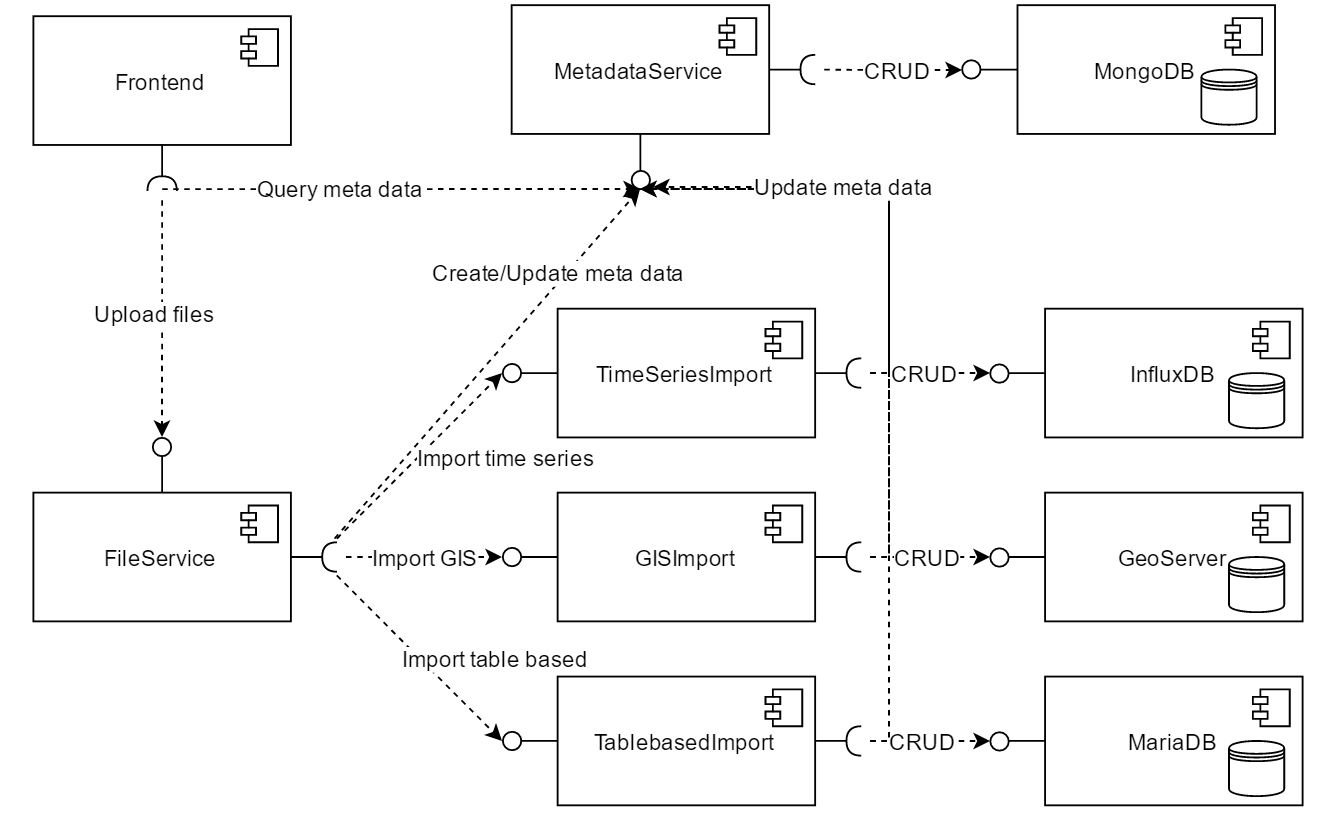
\includegraphics[width=1\textwidth]{./Images/ImportServices}
    \caption{Diagramm der Komponenten für die Import Services}
    \label{fig:ImportServices}
\end{figure}

Wie in der Abbildung \ref{fig:ImportServices} zu den Import Services gut erkenntlich interagieren alle Services, die für den Import zuständig sind, mit dem Service Metadata. Der Service Metadata hat die Aufgaben für die einzelne Dateien, die importiert werden, Metadata zu erstellen, zu aktualisieren und ggf. zu löschen. Die erstellten Metadata werden dann in einer Datenbank abgelegt. Dazu kann das Frontend via des Services Metadata auf die einzelnen Metadata zugreifen. Damit nicht jeder Service, der mit dem Service Metadata interagiert die Aufrufe selber implementieren muss und damit ggf. Redundanzen erzeugt, ist die Kommunikation mit dem Service Metadata im Objekt Metadata-Client gekapselt. Wenn eine Interaktion mit dem Service Metadata erforderlich ist, wird das Objekt Metadata-Client erzeugt, welches dann die Interaktionen übernimmt.

\subsection{Testumgebung}
Die verwendete Testumgebung ist sehr ähnlich zu der Testumgebung im Grundprojekt. Jedoch wurde nicht mehr mit einer virtuellen Maschine gearbeitet, da der VM nicht genug Leistung zugeteilt werden konnte. Daher wurde Linux Ubuntu als Host-System verwendet. Dies bedeutet aber auch, dass kein geschlossenes System mehr für das Testen verwendet wurde. 

Zudem wurde wieder Docker in Verbindung mit dem Tool Docker-Compose verwendet, da das Ausführen von MARS ohne Docker nicht möglich ist. Die Installation von MARS erfolgte nach der gleichen Vorgehensweise, wie im Grundprojekt. 

Ähnlich wie im Grundprojekt wurde auf einem GIT Branch gearbeitet und zwar wurde von den Import-Projekten ein Branch erstellt. Zum Zeitpunkt der Untersuchung von PACT innerhalb von MARS, gab es laufend Änderungen an den Services für den Import. Dies betraff teilweise auch die Schnittstelle. Um sich ausschließlich auf die Einbindung von PACT zu konzentrieren, wurde der Brach erstellt, damit keine Änderungen diesen Prozess beeinträchtigen können.

Für die Implementierung von PACT wurde Intellij als Entwicklungsumgebung verwendet. Dazu wurde Maven als Build-Management-Tool verwendet, da alle MARS-Projekte Maven verwenden und eine Umstellung auf Gradle zu viel Ressourcen verbraucht hätten, ohne vornhinein ermitteln zu können, ob es sich dadurch Vorteile ergeben. Ergänzend dazu wurden die Entwicklungswerkzeuge von Chromium und das Programm Postman verwendet, um die Interaktionen besser zu verstehen und MARS mit default Werten zu füllen. Postman ist ein Programm zum Erstellen, Testen und Dokumentieren von APIs. Zusätzlich wurde ein Framework für die Erstellung von Mocks verwendet und zwar das Framework Mockito.
\subsection{Einbindung in MARS}
Zwischen dem Metadata-Client und Metadata gibt es mehrere verschiedene Interaktionen. Dabei sind alle CRDU-Methoden, also GET,POST,PUT und DELETE, vertreten. Bei der Implementierung von PACT wurden jedoch nicht alle Interaktionen umgesetzt, da es zu aufwendig gewesen wäre. In der Tabelle \ref{tab:Interaktionen_PACT} auf der Seite \pageref{tab:Interaktionen_PACT} sind die Interaktionen kurz beschrieben, welche mit PACT implementiert werden sollten.

\begin{table}[htbp]
\centering
\begin{tabular}{|c|l|p{4cm}|p{4cm}|}
\hline
\multicolumn{1}{|l|}{Methode} & Beschreibung \\ \hline
GET & Bekomme einen Metadata-Eintrag via der spezifischen DataID zurück\\ \hline
GET & Bekomme alle Metadata-Einträge zurück \\ \hline
PUT & Aktualisiere die Variable, die den aktuellen Zustand des Uploads beschreibt \\ \hline
POST & Erstelle einen neuen Metadata-Eintrag \\ \hline
DELETE & Lösche einen Metadata-Eintrag via DataID\\ \hline
\end{tabular}
\caption{Interaktionen, die mit PACT umgesetzt wurden sind}
\label{tab:Interaktionen_PACT}
\end{table}

Als Soll-Zusand für die Tests wurden der Zustand genommen, der bei der Erstellung des Branches vorlag. Mithilfe dieses Soll-Zustandes wurden die Interaktionen in PACT implementiert. Als vorbereitetete Schrit davor, mussten die Interaktionen genaur analysiert werden, damit klar definiert werden kann, wie die Anfrage und die dazu gehörige Antwort auszusehen hat.


Der Zustand der Services besonders der Interaktionen 

Definieren welche Interaktionen mit PACT getestet werdewn sollen. Swagger.io, Postman und Chromium hilfreich
Anfrage und Antwort definieren, Jetzt-Zustand als Soll-Zustand

\subsubsection{Implementierung des Consumers}
Erster Implementierung ausführlich, Probleme beim Definieren des Body, und dann eine Methode nach der anderen

\subsubsection{Implementierung Provider}

\subsection{Untersuchung}


\begin{itemize}
\item Beschreibung der Testumgebung
\item Ziel beschrieben
\item Aussuchen eines Services und Consumers
\item Aufrufen herausfinden via Browser und Postman + Swagger
\item Testen der Aufrufe via Postman, um festzustellen das sie funktionieren und koirrekt sind
\item Aktueller Stand als korrekt anzusehen und Soll-Zustand
\item Branch
\item Implementierung des Consumers
\end{itemize}

\subsection{Fazit}
\begin{itemize}
\item Erklärung
\item Erläuterung zu der Verbindung mit Microservice
\item Normale Implementierung
\item Einbinden in Mars
\item Fazit
\end{itemize}
\section{Ausblick Masterarbeit}



\bibliography{literatur}
\bibliographystyle{alpha}

\end{document}